\section{Introdução}

\begin{frame}{Material de apoio}
    \fbox{
        \parbox{\linewidth}{
        \$ git clone --recursive \\ https://github.com/AndreKuru/Minicurso-Vim.git
        }
    }

    \vfill

    \hyperlink{https://media.pragprog.com/titles/dnvim2/code/dnvim2-code.zip}{pratical-vim-examples}
\end{frame}

\begin{frame}{Vim}
    \begin{columns}
        \begin{column}{0.3\textwidth}
            \begin{figure}
                \centering
                
\includegraphics[height=0.6\linewidth]{Image/vi-logo.png}
                \label{vi-logo}
            \end{figure}
        \end{column}
        
        \begin{column}{0.3\textwidth}
            \begin{figure}
                \centering
                
\includegraphics[height=0.6\linewidth]{Image/vim-logo.png}
                \label{vim-logo}
            \end{figure}
        \end{column}
        
        \begin{column}{0.3\textwidth}
            \begin{figure}
                \centering
                
\includegraphics[height=0.6\linewidth]{Image/neovim-logo.png}
                \label{neovim-logo}
            \end{figure}
        \end{column}
        
    \end{columns}
\end{frame}

\begin{frame}{Principais modos}
    \begin{wideitemize}
        \item \textbf{Normal}: navegar e editar
        \item \textbf{Insert}: inserção de texto
        \item \textbf{Visual}: editar através de seleção
        \item \textbf{Command-line}: retentor de usuários de primeira viagem
    \end{wideitemize}
\end{frame}

\begin{frame}{Digitação ideal}
    \begin{figure}
        \centering
        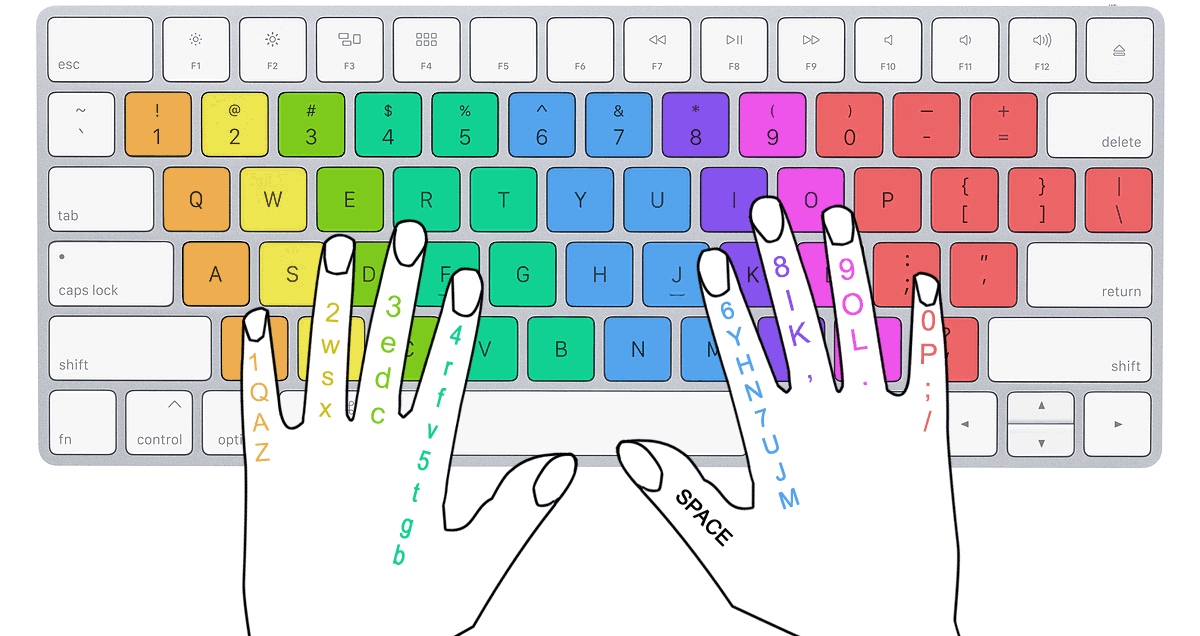
\includegraphics[width=\linewidth]{Image/Finger_position_on_a_keyboard.png}
        \label{finger-position}
        \footnotesize
        \\ Imagem não adaptada. \\
        Disponível em:  \hyperlink{https://commons.wikimedia.org/wiki/File:Finger_position_on_a_keyboard.png}{Wikimedia}
    \end{figure}
\end{frame}


\begin{frame}{Movimentação básica}
    \begin{columns}
        \begin{column}{0.4\textwidth}
            \begin{widedescription}
                \item \key{j}: $\downarrow$
                \item \key{k}: $\uparrow$
                \item \key{l}: $\rightarrow$
                \item \key{h}: $\leftarrow$
                \item Jogo para praticar: \\ \hyperlink{https://vim-adventures.com/}{vim-adventures.com}
            \end{widedescription}
        \end{column}
        
        \begin{column}{0.6\textwidth}
            \begin{figure}
                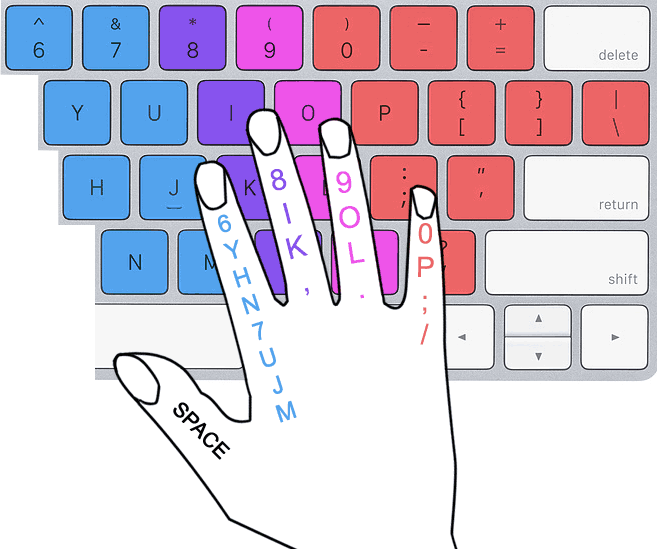
\includegraphics[width=\linewidth]{Image/Finger_position_on_a_keyboard-only-right-hand.png}
                \label{right-hand} 
                \footnotesize
                \\ Imagem adaptada. \\
                Disponível em:  \hyperlink{https://commons.wikimedia.org/wiki/File:Finger_position_on_a_keyboard.png}{Wikimedia}
            \end{figure}
        \end{column}
    \end{columns}

    \begin{flushleft}
    \end{flushleft}
\end{frame}

\begin{frame}{Quando não se precisa manter a mão no mouse}
    \begin{columns}
        \begin{column}{0.4\linewidth}
            \begin{wideitemize}
                \item \key{u}: \textbf{u}ndo change
                \item \key{dd}: \textbf{d}elete line
                \item \key{yy}: \textbf{y}ank line
                \item \key{p}: \textbf{p}ut text
            \end{wideitemize}
        \end{column}
        
        \begin{column}{0.3\textwidth}
            \begin{figure}
                
\includegraphics[width=\linewidth]{Image/kelly-sikkema-K5dAn1gOFEc-unsplash.jpg}
                \footnotesize
                \\ Imagem não adaptada. \\
                Disponível em:  \hyperlink{https://unsplash.com/photos/person-using-black-and-silver-laptop-computer-K5dAn1gOFEc}{Unsplash}
            \end{figure}
        \end{column}
        
        \begin{column}{0.3\textwidth}
            \begin{widedescription}
                \item Mas se quiser pode
                \item \key{:set mouse=a}
            \end{widedescription}
        \end{column}
    \end{columns}
\end{frame}

\begin{frame}{Experimentando cada modo}
    \begin{wideitemize}
        \item \key{i}: switch to \textbf{I}nsert mode
        \item \key{v}: switch to \textbf{V}isual mode
        \item \key{:}: switch to Command-Line mode
    \end{wideitemize}
\end{frame}

\begin{frame}{Como sair do vim?}
    \begin{widedescription}
        \item \key{:q}: \textbf{q}uit
        \item \key{:q!}: \textbf{q}uit without writing
        \item \key{:w}: \textbf{w}rite
        \item \key{:wq}: \textbf{w}rite and \textbf{q}uit
        \item \key{:x}: write (if needed) and quit
    \end{widedescription}
\end{frame}